\documentclass[]{article}
\usepackage{lmodern}
\usepackage{setspace}
\setstretch{1}
\usepackage{amssymb,amsmath}
\usepackage{ifxetex,ifluatex}
\usepackage{fixltx2e} % provides \textsubscript
\ifnum 0\ifxetex 1\fi\ifluatex 1\fi=0 % if pdftex
  \usepackage[T1]{fontenc}
  \usepackage[utf8]{inputenc}
\else % if luatex or xelatex
  \ifxetex
    \usepackage{mathspec}
  \else
    \usepackage{fontspec}
  \fi
  \defaultfontfeatures{Ligatures=TeX,Scale=MatchLowercase}
\fi
% use upquote if available, for straight quotes in verbatim environments
\IfFileExists{upquote.sty}{\usepackage{upquote}}{}
% use microtype if available
\IfFileExists{microtype.sty}{%
\usepackage{microtype}
\UseMicrotypeSet[protrusion]{basicmath} % disable protrusion for tt fonts
}{}
\usepackage[margin=1in]{geometry}
\usepackage{hyperref}
\hypersetup{unicode=true,
            pdftitle={Ohio CAUV Value Projections for 2019 and 2020},
            pdfauthor={Robert Dinterman and Ani L. Katchova},
            pdfborder={0 0 0},
            breaklinks=true}
\urlstyle{same}  % don't use monospace font for urls
\usepackage{longtable,booktabs}
\usepackage{graphicx,grffile}
\makeatletter
\def\maxwidth{\ifdim\Gin@nat@width>\linewidth\linewidth\else\Gin@nat@width\fi}
\def\maxheight{\ifdim\Gin@nat@height>\textheight\textheight\else\Gin@nat@height\fi}
\makeatother
% Scale images if necessary, so that they will not overflow the page
% margins by default, and it is still possible to overwrite the defaults
% using explicit options in \includegraphics[width, height, ...]{}
\setkeys{Gin}{width=\maxwidth,height=\maxheight,keepaspectratio}
\IfFileExists{parskip.sty}{%
\usepackage{parskip}
}{% else
\setlength{\parindent}{0pt}
\setlength{\parskip}{6pt plus 2pt minus 1pt}
}
\setlength{\emergencystretch}{3em}  % prevent overfull lines
\providecommand{\tightlist}{%
  \setlength{\itemsep}{0pt}\setlength{\parskip}{0pt}}
\setcounter{secnumdepth}{0}
% Redefines (sub)paragraphs to behave more like sections
\ifx\paragraph\undefined\else
\let\oldparagraph\paragraph
\renewcommand{\paragraph}[1]{\oldparagraph{#1}\mbox{}}
\fi
\ifx\subparagraph\undefined\else
\let\oldsubparagraph\subparagraph
\renewcommand{\subparagraph}[1]{\oldsubparagraph{#1}\mbox{}}
\fi

%%% Use protect on footnotes to avoid problems with footnotes in titles
\let\rmarkdownfootnote\footnote%
\def\footnote{\protect\rmarkdownfootnote}

%%% Change title format to be more compact
\usepackage{titling}

% Create subtitle command for use in maketitle
\providecommand{\subtitle}[1]{
  \posttitle{
    \begin{center}\large#1\end{center}
    }
}

\setlength{\droptitle}{-2em}

  \title{Ohio CAUV Value Projections for 2019 and 2020}
    \pretitle{\vspace{\droptitle}\centering\huge}
  \posttitle{\par}
  \subtitle{Department of Agricultural, Environmental and Development Economics,\\
The Ohio State University}
  \author{Robert Dinterman\footnote{Post-Doctoral Researcher} and Ani L.
Katchova\footnote{Associate Professor and Farm Income Enhancement Chair}}
    \preauthor{\centering\large\emph}
  \postauthor{\par}
      \predate{\centering\large\emph}
  \postdate{\par}
    \date{2019-05-02}

\usepackage{floatrow}
\floatsetup[figure]{capposition=top}

\begin{document}
\maketitle

\hypertarget{key-findings}{%
\section{Key Findings}\label{key-findings}}

The purpose of this report is to provide projections of property tax for
agricultural land in Ohio for tax years 2019 and 2020. The projections
apply for all soil types in Ohio enrolled in the Current Agricultural
Use Value Program (CAUV). Further, the CAUV formula that is used to
calculate CAUV values based on soil types is explained, along with the
components of the formula and the assumptions that are used to make
expected, high, and low CAUV value projections for 2019 and 2020.
Legislation passed in 2017 altered CAUV calculations, which are detailed
in this report. We explain the current methodology for calculating CAUV
values and how these projections were made. We used Ohio Department of
Taxation (ODT) descriptions of calculations, the
\href{http://codes.ohio.gov/orc/5713.31}{Ohio Code of legislation} on
CAUV, and the \href{http://codes.ohio.gov/orc/5715.01}{phase-in
legislation} for the new calculations.

\textbf{Key Findings}

\begin{itemize}
\tightlist
\item
  Project a decrease in the average CAUV value across all soil types in
  Ohio to approximately \$870 in the 2019 tax year. This represents a
  -14\% change from the average 2018 CAUV value of \$1,015.
\item
  The 2019 tax year is the third year of the phase-in from large-scale
  changes in the calculation of CAUV values. If the phase-in procedure
  was not in place, then the average 2019 CAUV values would have further
  dropped to approximately \$730.
\item
  Due to uncertainty in finalized input data used in our 2019 CAUV
  calculations, it is possible for the average CAUV value to change from
  2018 average CAUV value by as much as -23\% while it is also possible
  for the average CAUV value to rise by over 27\%. However, an increase
  in CAUV values for 2019 is unlikely.
\item
  Current CAUV projections for the 2020 tax year, which represents the
  first year without the phased-in procedure, expects a further decline
  in the average CAUV value to \$585 which would be a 14\% change from
  current projections in 2019.
\item
  Due to uncertainty in finalized input data used in our 2020 CAUV
  calculations, it is possible for the average CAUV value to change from
  2019 average CAUV value by as much as -42\% while it is also possible
  for the average CAUV value to rise by over 6\%. However, an increase
  in CAUV values for 2020 is unlikely.
\end{itemize}

\newpage
\setstretch{1.5}

\hypertarget{cauv-value-projections-for-2019-and-2020}{%
\section{CAUV Value Projections for 2019 and
2020}\label{cauv-value-projections-for-2019-and-2020}}

In 2018, the average CAUV value across all soil types was \$1,015 per
Ohio Department of Taxation (ODT). Our projection for the average value
of CAUV in the 2019 tax year is \$872. Our projections are partially
based on how the CAUV formula use Olympic averaging\footnote{A 7-year
  Olympic average is a mean of the previous 7 values after first
  removing the highest and lowest values from calculation. For
  projections, we assume the most recent data is either the
  highest/lowest value in the 7 year span.} for certain components and
it is possible for a potential high of \$1,287 and a low of \$787 for
average CAUV values. However, it is unlikely to have large divergence
from our expected projections based on the currently available data for
components which use Olympic averaging.

Updates to CAUV values do not occur equally across Ohio as there is a
rotating schedule for tax assessments in Ohio.
\href{https://www.tax.ohio.gov/real_estate/reappraisal_and_triennial_update.aspx}{Once
every six years}, a county receives a full reappraisal of their property
with an adjustment in the third year in between. Each county receives an
update to their CAUV values for the years a reappraisal or adjustment
occurs. About a quarter of the state received a CAUV value update in
2018, another quarter in 2019, and about half of the state will see
updates in 2020. Figure \ref{fig:update-map} provides a reference for
when a county receives an update to their CAUV values:

\begin{figure}[H]
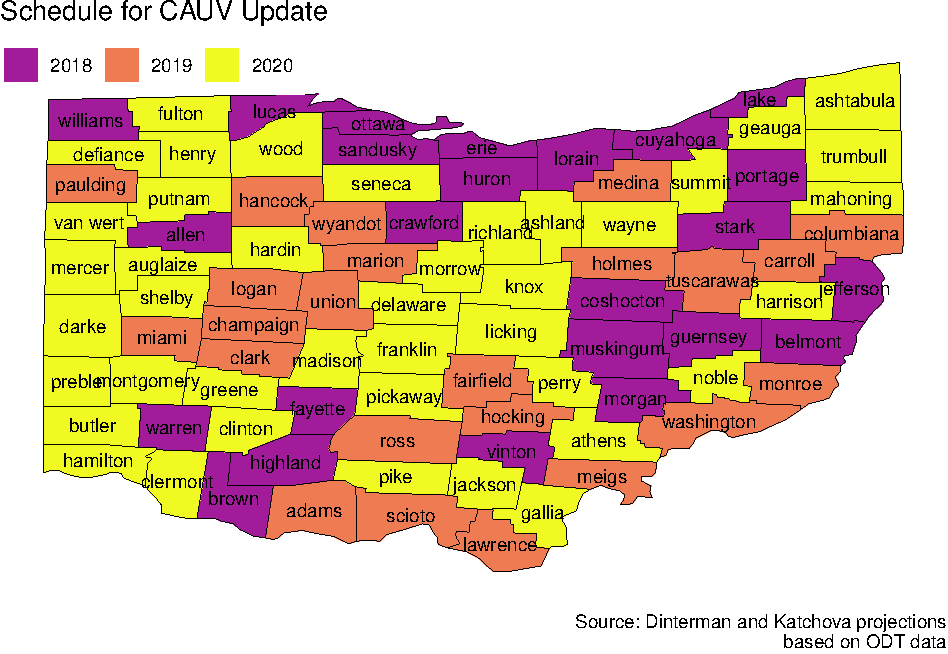
\includegraphics[width=1\linewidth]{4-projections-2019-2020_files/figure-latex/update-map-1} \caption{\label{fig:update-map}}\label{fig:update-map}
\end{figure}

CAUV values contain 5 major components used as inputs for projecting
values: capitalization rate, commodity yields, commodity prices,
commodity acreage/rotation, and non-land input costs. The commodities
used in CAUV are corn, soybeans, and wheat. Each of these components are
projected into the future to obtain the projections for 2019 and 2020
CAUV values.

Our projections for the CAUV values in the 2019 tax year are for the
components of commodity yields, commodity rotation, and capitalization
rate to remain largely unchanged from 2018. Input costs are expected to
decline, although this is counteracted with commodity prices similarly
expected to decline. Under the expected scenario, the average CAUV value
will continue to decline by a similar proportion as the fall in the CAUV
values from 2016 to 2017 and then to 2018. Grouping soil types based on
a productivity index can help display how similarly productive soils are
expected to decline in our 2019 projections:

\begin{figure}[H]
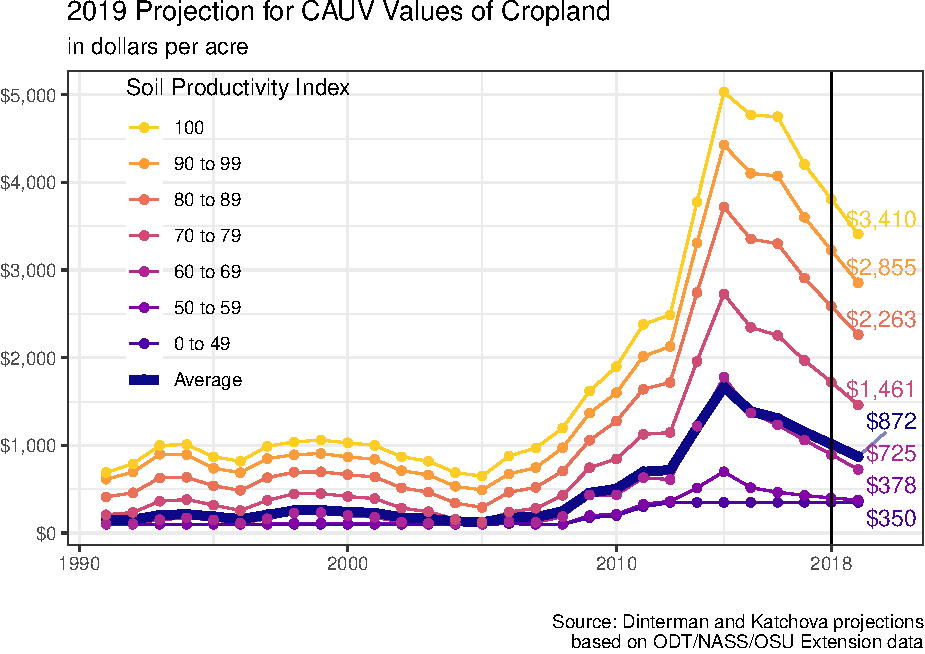
\includegraphics[width=1\linewidth]{4-projections-2019-2020_files/figure-latex/exp-trend-1} \caption{\label{fig:exp-trend}}\label{fig:exp-trend}
\end{figure}

The projected CAUV values are partially offset by the current provision
in the CAUV calculations that phases in the new formula for CAUV,
smoothing the adjustment to lower CAUV values the one cycle of property
reassessment rather than these declines occurring immediately. The 2018
values had an adjustment factor where only half of the difference was
included between the 2017 CAUV value and what the pre-adjusted 2018 CAUV
would have been. This also occurs for 2019, where if the calculated CAUV
value in 2019 is lower than the 2018 CAUV value for a soil type then
only half of the difference is factored into the actual 2019 CAUV value.
While the projected average CAUV value for 2019 is \$872, the value
would have been \$729 without the phase-in. Figure \ref{fig:exp-2019}
shows how much this adjustment for phasing in of the new calculations
differ by soil types:

\begin{figure}[H]
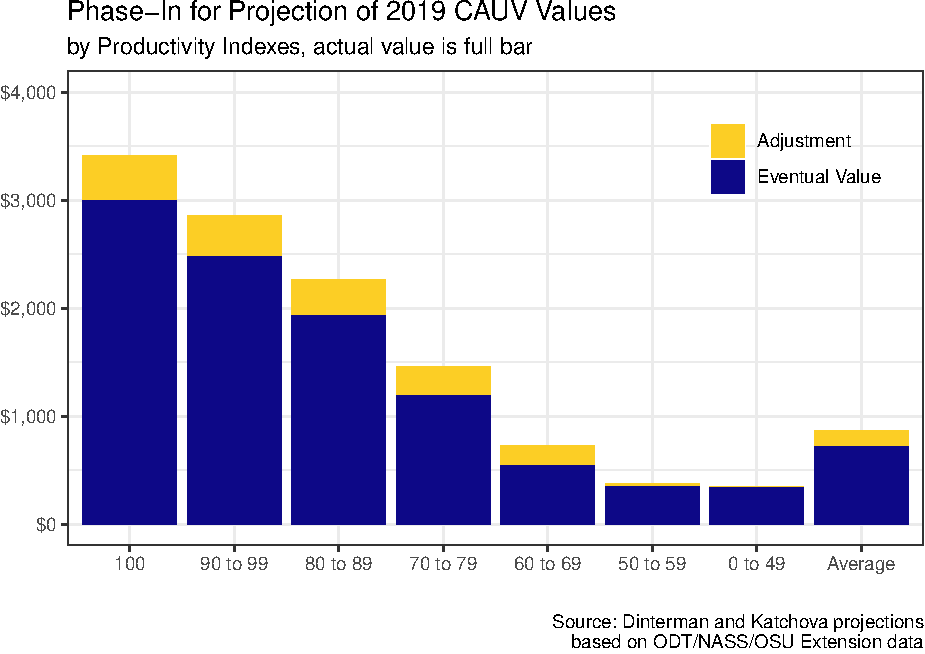
\includegraphics[width=1\linewidth]{4-projections-2019-2020_files/figure-latex/exp-2019-1} \caption{\label{fig:exp-2019}}\label{fig:exp-2019}
\end{figure}

This adjustment procedure will not be present in tax year of 2020 and
beyond as the phase-in was only intended to affect one one set of
phased-in values based on the triennial update of property assessments.
Because of this, we have further pushed our projections for the 2020 tax
year by extending each component in the CAUV calculation an additional
year with as much of the available data as possible.

Our preliminary results indicate stable values for commodity yields,
commodity rotation, and capitalization to remain similar to our
projections for 2019. Further, the input costs and commodity prices are
anticipated to further decline with a more pronounced decline for prices
than input costs. At this time, our expected projections for the 2020
tax year are:

\begin{figure}[H]
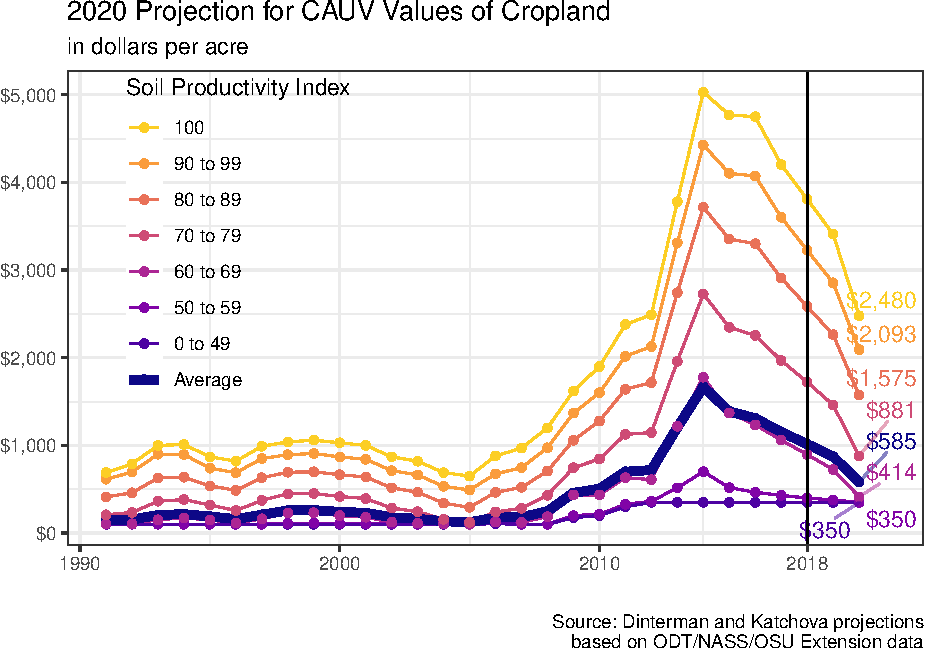
\includegraphics[width=1\linewidth]{4-projections-2019-2020_files/figure-latex/exp-trend-2020-1} \caption{\label{fig:exp-trend-2020}}\label{fig:exp-trend-2020}
\end{figure}

\newpage

\hypertarget{current-agricultural-use-value-program-overview}{%
\section{Current Agricultural Use Value Program
Overview}\label{current-agricultural-use-value-program-overview}}

In 1974, Ohio enacted the Current Agricultural Use Value Program (CAUV)
as a tax incentive for farmers to continue agricultural production on
their land instead of selling it due to urbanization pressure. CAUV
provides an appraisal method for valuing agricultural land by use of
only agricultural inputs rather than the market value of land.
Throughout the 1970s, other states adopted similar programs of
differential appraisal methods of agricultural land and, as of 2014, all
50 states within the US provide some form of differential tax treatment
of agricultural land. While each state has its own reason for enacting
preferential tax treatment and its particular calculation, the intent
behind differential taxation is generally understood as applying a net
present valuation of agricultural production that is not tied to
potential urbanization development pressures. Ohio is no different and
has developed its own calculation method that depends on soil quality,
commodity yields/prices/rotation, operational costs, and capitalization
rate. The basic premise has been in place since the late 1970s although
the program has become more sophisticated and received substantial
updates in 2006, 2015, and most recently in 2017 that have affected the
calculation of CAUV.

No matter what commodity a farmer produces, their CAUV value is
determined solely based on their soil type and a formula from the Ohio
Department of Taxation (ODT) which aims to represent the expected
returns for an average farmer in Ohio. A simplified version of the
calculation can be stated as:

\begin{quote}
The CAUV value is the expected net present value of an acre of land
based on expected net income of the land used for agricultural purposes.
To determine this, first a historical average of yields and prices for
corn, soybeans, and wheat is used to determine gross income. Then
historical non-land costs -- provided by The Ohio State University
Extension -- are subtracted from gross income for a measure of net
income. And finally, this net income is divided by a capitalization rate
based upon historical values of farm interest and equity rates. This
CAUV value will vary based upon the particular soil type(s) for a farm.
\end{quote}

For agricultural land to be eligible for CAUV, it must either be at
least 10 acres devoted exclusively to commercial agricultural use or be
able to produce more than \$2,500 in average gross income. The general
trend for the state of Ohio since the 1980s has been a steady increase
in the total acreage enrolled in CAUV, although there have been declines
in enrolled CAUV acreage for areas under urbanization pressure as
farmland is converted to residential or commercial purposes. When a land
owner decides to unenroll from CAUV for this purpose, they must pay a
recoupment penalty that is equal to the CAUV tax savings for the
previous 3 tax years -- i.e.~the difference between the market value and
CAUV value.

\hypertarget{cauv-value-formula}{%
\subsection{CAUV Value Formula}\label{cauv-value-formula}}

For each of the over 3,500 soil types (\(s\)) in Ohio, a particular
year's (\(t\)) CAUV value is calculated as the soil's net income divided
by the capitalization rate:

\[
CAUV_{s,t} = \frac{NOI_{s,t}}{CAP_t} \label{eq:cauv}
\]

where \(CAP_t\) represents the capitalization rate and \(NOI_{s,t}\)
represents the net operating income based on revenues less non-land
costs for corn, soybeans, and wheat.

\hypertarget{net-operating-income}{%
\subsection{Net Operating Income}\label{net-operating-income}}

Net operating income, \({NOI_{s,t}}\), captures the average returns to
an acre of land under normal management practices which is adjusted by
the state-wide rotation pattern of commodities. In other words, a net
income for corn, soybeans, and wheat is calculated for each soil type
and then these net incomes for a given soil type are averaged in
proportion to the state-wide acreage of harvested corn, soybeans, and
wheat. This can be defined as:

\[
NOI_{s,t} = \sum_{c} w_{c,t}\times(GOI_{s,c,t} - {non-land}_{s,c,t})
\]

where \(c\) denotes the commodity type, which is either corn, soybeans,
or wheat which represent the dominant commodities in Ohio and
\(w_{c,t}\) is commodity's share of state production. \(GOI_{s,c,t}\) is
the gross operating income for a soil type and is calculated for each of
the commodity types (corn, soybeans, and wheat) based on yields and
prices. \({non-land}_{s,c,t}\) is the non-land costs associated with
each commodity type. Both of these variables are further explained in
the following sections.

\hypertarget{rotation}{%
\subsubsection{Rotation}\label{rotation}}

Each commodity's share of state production is based on a 5-year average
of total acres harvested between the three commodities -- with weights
summing to 1. This is done by summing up the total harvested acreage for
corn, for soybeans, and for wheat over the past six years ignoring the
current -- i.e.~2019 value for CAUV calculations uses 2014 to 2018
harvested acres. Once summed up, each commodity is then assigned their
share of total harvested for the entire state based on those past six
years ignoring the current.

These data are from the United States Department of Agriculture (USDA)
\href{https://usda.mannlib.cornell.edu/MannUsda/viewDocumentInfo.do?documentID=1046}{Crop
Production Reports}. Typically there is an August, September, October,
and November forecast for Ohio's corn, soybeans, and wheat acreage with
the
\href{https://usda.mannlib.cornell.edu/MannUsda/viewDocumentInfo.do?documentID=1047}{finalized
values} occurring in January of the following year -- i.e.~2018
harvested acres was finalized in January 2019. The values are lagged one
year -- the 2019 values for commodity rotation percentages are based on
the 2014 through 2018 harvested acreage which is known at this time but
the 2020 value will will use the 2018 harvested acreage for a
preliminary estimate of 2019 harvested acreage.

The values of rotation used in ODT calculations since 2010 are displayed
in the following tables along with the values used in our 2019 and 2020
CAUV value projections.

\begin{longtable}[]{@{}rllll@{}}
\caption{Historical Corn Rotation}\tabularnewline
\toprule
Year & ODT Value & USDA Acres Harvested & AVG Acres Harvested &
Projected\tabularnewline
\midrule
\endfirsthead
\toprule
Year & ODT Value & USDA Acres Harvested & AVG Acres Harvested &
Projected\tabularnewline
\midrule
\endhead
2010 & 39.0\% & 3,270,000 & 3,210,000 & 37.7\%\tabularnewline
2011 & 38.6\% & 3,200,000 & 3,216,000 & 37.7\%\tabularnewline
2012 & 38.6\% & 3,650,000 & 3,220,000 & 37.7\%\tabularnewline
2013 & 38.7\% & 3,740,000 & 3,268,000 & 38.1\%\tabularnewline
2014 & 38.6\% & 3,480,000 & 3,276,000 & 38.1\%\tabularnewline
2015 & 40.0\% & 3,260,000 & 3,468,000 & 40.2\%\tabularnewline
2016 & 40.2\% & 3,300,000 & 3,466,000 & 40.1\%\tabularnewline
2017 & 40.0\% & 3,150,000 & 3,486,000 & 40.3\%\tabularnewline
2018 & 39.0\% & 3,300,000 & 3,386,000 & 39.0\%\tabularnewline
2019 & NA\% & NA & 3,298,000 & 38.0\%\tabularnewline
2020 & NA\% & NA & 3,264,639 & 37.6\%\tabularnewline
\bottomrule
\end{longtable}

\begin{longtable}[]{@{}rllll@{}}
\caption{Historical Soy Rotation}\tabularnewline
\toprule
Year & ODT Value & USDA Acres Harvested & AVG Acres Harvested &
Projected\tabularnewline
\midrule
\endfirsthead
\toprule
Year & ODT Value & USDA Acres Harvested & AVG Acres Harvested &
Projected\tabularnewline
\midrule
\endhead
2010 & 51.0\% & 4,590,000 & 4,448,000 & 52.2\%\tabularnewline
2011 & 50.9\% & 4,540,000 & 4,470,000 & 52.4\%\tabularnewline
2012 & 51.1\% & 4,590,000 & 4,492,000 & 52.6\%\tabularnewline
2013 & 51.2\% & 4,490,000 & 4,476,000 & 52.2\%\tabularnewline
2014 & 52.0\% & 4,690,000 & 4,546,000 & 52.9\%\tabularnewline
2015 & 52.6\% & 4,740,000 & 4,580,000 & 53.1\%\tabularnewline
2016 & 53.0\% & 4,840,000 & 4,610,000 & 53.4\%\tabularnewline
2017 & 54.0\% & 5,090,000 & 4,670,000 & 53.9\%\tabularnewline
2018 & 55.0\% & 4,980,000 & 4,770,000 & 55.0\%\tabularnewline
2019 & NA\% & NA & 4,868,000 & 56.1\%\tabularnewline
2020 & NA\% & NA & 4,919,894 & 56.7\%\tabularnewline
\bottomrule
\end{longtable}

\begin{longtable}[]{@{}rllll@{}}
\caption{Historical Wheat Rotation}\tabularnewline
\toprule
Year & ODT Value & USDA Acres Harvested & AVG Acres Harvested &
Projected\tabularnewline
\midrule
\endfirsthead
\toprule
Year & ODT Value & USDA Acres Harvested & AVG Acres Harvested &
Projected\tabularnewline
\midrule
\endhead
2010 & 10.0\% & 700,000 & 900,000 & 10.6\%\tabularnewline
2011 & 10.5\% & 850,000 & 912,000 & 10.7\%\tabularnewline
2012 & 10.3\% & 450,000 & 886,000 & 10.4\%\tabularnewline
2013 & 10.1\% & 640,000 & 864,000 & 10.1\%\tabularnewline
2014 & 9.4\% & 545,000 & 808,000 & 9.4\%\tabularnewline
2015 & 7.4\% & 480,000 & 637,000 & 7.4\%\tabularnewline
2016 & 6.8\% & 560,000 & 593,000 & 6.9\%\tabularnewline
2017 & 6.0\% & 460,000 & 535,000 & 6.2\%\tabularnewline
2018 & 6.0\% & 450,000 & 537,000 & 6.2\%\tabularnewline
2019 & NA\% & NA & 499,000 & 5.7\%\tabularnewline
2020 & NA\% & NA & 486,947 & 5.6\%\tabularnewline
\bottomrule
\end{longtable}

\hypertarget{non-land-cost}{%
\subsubsection{Non-Land Cost}\label{non-land-cost}}

The non-land costs are calculated as 7-year Olympic averages for typical
costs of producing each commodity (corn, soybeans, and wheat). The
\href{https://farmoffice.osu.edu/farm-management-tools/farm-budgets}{Farm
Office} at The Ohio State University Extension conducts annual surveys
for costs of production which serve as the yearly estimates that are
used in the 7-year Olympic average. Budgets for a commodity marketing
year are generally released in October of the prior year and then
finalized in May of the marketing year -- i.e.~the 2019 marketing year
was initially released in October 2018 and will likely be finalized
sometime after May 2019. These budgets will include both fixed
(machinery, equipment, labor, etc.) and variable (seeds, fertilizer,
chemicals, hauling, etc.) costs involved in producing corn, wheat, or
soybeans and each of these individual components are averaged for use in
CAUV calculation.

Prior to 2015, the non-land costs were lagged one year -- i.e.~tax year
2014 used the values from budgets in 2007 to 2013. From 2015 onward, the
current year values are included in the non-land cost calculations.
Because of the nature of an Olympic average, the non-land costs used in
2019 CAUV is bounded between a ``high'' and a ``low'' value by averaging
the previous 6-years after dropping only the highest or lowest value
respectively. In the event that the ``high'' value of our projected
non-land costs occur, then this is where the 2019 non-land costs are all
the lowest values in the previous 7-years which causes the CAUV to be a
higher value. The opposite is true for the ``low'' value in that the
non-land costs are all 7-year highs.

Our projection of non-land base costs for corn is \$519; for soybeans is
\$339; and for wheat is \$320 per acre for 2019. For 2020, our
projections are \$500 for corn; \$330 for soybeans; and \$308 for wheat.
The historical and projected values for each commodity are displayed in
figure \ref{fig:viz-nonland}:

\begin{figure}[H]
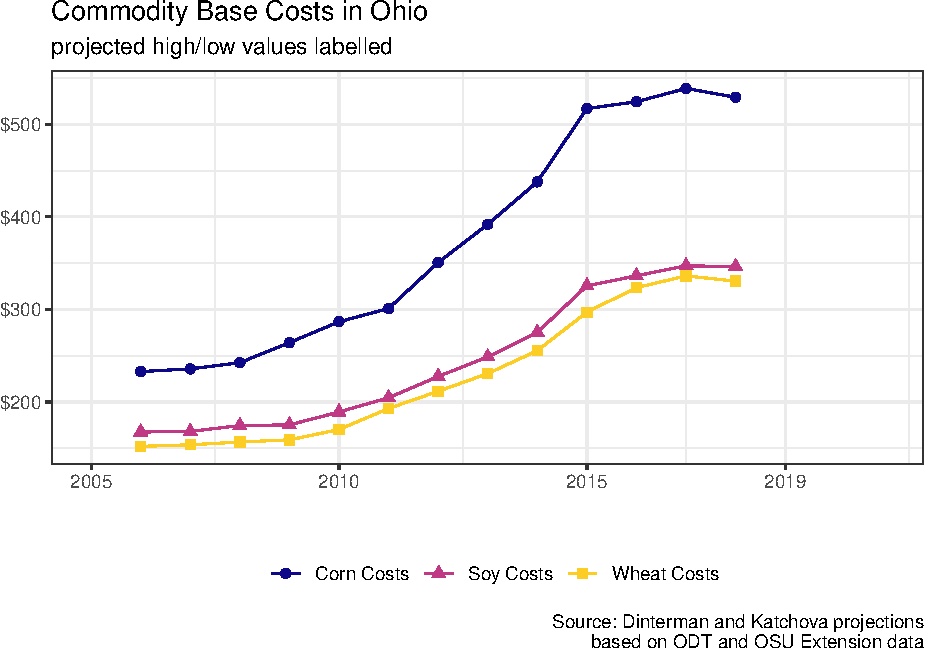
\includegraphics[width=1\linewidth]{4-projections-2019-2020_files/figure-latex/viz-nonland-1} \caption{\label{fig:viz-nonland}}\label{fig:viz-nonland}
\end{figure}

A base cost is assigned for each commodity and is the same across all
soil types. The base cost has an associated base yield for each
commodity, which is calculated from the budget reports of OSU Extension.
However, each soil type has an associated expected yield (explained in
the following section) and there is an adjustment applied for each
commodity if the expected yield is above or below the base yield. Each
additional yield above or below the base yield is multiplied by an
additional cost per yield -- which is calculated in the same manner as
the base costs with a 7-year Olympic average. However, these additional
costs vary across soil types which makes it difficult to present for all
soil types.

However, we also calculate hypothetical high or low scenarios for this
year as a way to place bounds on the non-land costs of each commodity.
The base and additional costs for all commodities are displayed in
tables on the following pages with the associated ranges of the high or
low projections.

\newpage

\begin{longtable}[]{@{}rllll@{}}
\caption{Historical Corn Base Costs}\tabularnewline
\toprule
Year & ODT Base Cost & Projection & Low Projection & High
Projection\tabularnewline
\midrule
\endfirsthead
\toprule
Year & ODT Base Cost & Projection & Low Projection & High
Projection\tabularnewline
\midrule
\endhead
2013 & \$391.90 & \$393.31 & \$404.50 & \$348.09\tabularnewline
2014 & \$437.85 & \$438.22 & \$449.28 & \$388.52\tabularnewline
2015 & \$516.99 & \$518.46 & \$536.31 & \$483.59\tabularnewline
2016 & \$524.47 & \$526.74 & \$545.30 & \$502.49\tabularnewline
2017 & \$538.78 & \$540.77 & \$559.88 & \$521.58\tabularnewline
2018 & \$529.28 & \$532.45 & \$561.46 & \$527.62\tabularnewline
2019 & \$NA & \$519.19 & \$553.37 & \$509.98\tabularnewline
2020 & \$NA & \$500.25 & \$532.23 & \$493.05\tabularnewline
\bottomrule
\end{longtable}

\begin{longtable}[]{@{}rllll@{}}
\caption{Historical Corn Additional Costs}\tabularnewline
\toprule
Year & ODT Add Cost & Projection & Low Projection & High
Projection\tabularnewline
\midrule
\endfirsthead
\toprule
Year & ODT Add Cost & Projection & Low Projection & High
Projection\tabularnewline
\midrule
\endhead
2013 & \$1.04 & \$1.07 & \$1.16 & \$0.95\tabularnewline
2014 & \$1.18 & \$1.22 & \$1.28 & \$1.06\tabularnewline
2015 & \$1.36 & \$1.36 & \$1.44 & \$1.24\tabularnewline
2016 & \$1.38 & \$1.39 & \$1.44 & \$1.30\tabularnewline
2017 & \$1.45 & \$1.47 & \$1.54 & \$1.40\tabularnewline
2018 & \$1.44 & \$1.44 & \$1.52 & \$1.42\tabularnewline
2019 & \$NA & \$1.41 & \$1.53 & \$1.34\tabularnewline
2020 & \$NA & \$1.39 & \$1.49 & \$1.33\tabularnewline
\bottomrule
\end{longtable}

\newpage

\begin{longtable}[]{@{}rllll@{}}
\caption{Historical Soybeans Base Costs}\tabularnewline
\toprule
Year & ODT Base Cost & Projection & Low Projection & High
Projection\tabularnewline
\midrule
\endfirsthead
\toprule
Year & ODT Base Cost & Projection & Low Projection & High
Projection\tabularnewline
\midrule
\endhead
2013 & \$248.69 & \$247.71 & \$254.49 & \$222.50\tabularnewline
2014 & \$275.21 & \$273.55 & \$281.53 & \$245.24\tabularnewline
2015 & \$325.42 & \$326.03 & \$336.94 & \$304.40\tabularnewline
2016 & \$336.33 & \$336.63 & \$346.37 & \$317.49\tabularnewline
2017 & \$347.10 & \$346.25 & \$358.49 & \$332.90\tabularnewline
2018 & \$346.26 & \$346.69 & \$362.95 & \$338.83\tabularnewline
2019 & \$NA & \$338.88 & \$360.66 & \$330.01\tabularnewline
2020 & \$NA & \$329.95 & \$349.23 & \$322.37\tabularnewline
\bottomrule
\end{longtable}

\begin{longtable}[]{@{}rllll@{}}
\caption{Historical Soybeans Additional Costs}\tabularnewline
\toprule
Year & ODT Add Cost & Projection & Low Projection & High
Projection\tabularnewline
\midrule
\endfirsthead
\toprule
Year & ODT Add Cost & Projection & Low Projection & High
Projection\tabularnewline
\midrule
\endhead
2013 & \$1.12 & \$1.15 & \$1.29 & \$0.95\tabularnewline
2014 & \$1.27 & \$1.25 & \$1.43 & \$1.10\tabularnewline
2015 & \$1.24 & \$1.16 & \$1.33 & \$1.14\tabularnewline
2016 & \$1.07 & \$1.07 & \$1.14 & \$1.06\tabularnewline
2017 & \$1.05 & \$1.04 & \$1.13 & \$1.04\tabularnewline
2018 & \$0.94 & \$0.95 & \$1.03 & \$0.93\tabularnewline
2019 & \$NA & \$0.92 & \$0.99 & \$0.83\tabularnewline
2020 & \$NA & \$0.91 & \$0.96 & \$0.84\tabularnewline
\bottomrule
\end{longtable}

\newpage

\begin{longtable}[]{@{}rllll@{}}
\caption{Historical Wheat Base Costs}\tabularnewline
\toprule
Year & ODT Base Cost & Projection & Low Projection & High
Projection\tabularnewline
\midrule
\endfirsthead
\toprule
Year & ODT Base Cost & Projection & Low Projection & High
Projection\tabularnewline
\midrule
\endhead
2013 & \$230.62 & \$227.70 & \$235.39 & \$205.19\tabularnewline
2014 & \$255.48 & \$257.51 & \$268.56 & \$226.37\tabularnewline
2015 & \$296.98 & \$291.15 & \$302.89 & \$265.46\tabularnewline
2016 & \$323.52 & \$320.21 & \$330.25 & \$296.77\tabularnewline
2017 & \$336.21 & \$336.08 & \$348.08 & \$316.21\tabularnewline
2018 & \$330.53 & \$331.13 & \$349.74 & \$326.08\tabularnewline
2019 & \$NA & \$319.52 & \$341.07 & \$311.39\tabularnewline
2020 & \$NA & \$307.73 & \$328.28 & \$302.81\tabularnewline
\bottomrule
\end{longtable}

\begin{longtable}[]{@{}rllll@{}}
\caption{Historical Wheat Additional Costs}\tabularnewline
\toprule
Year & ODT Add Cost & Projection & Low Projection & High
Projection\tabularnewline
\midrule
\endfirsthead
\toprule
Year & ODT Add Cost & Projection & Low Projection & High
Projection\tabularnewline
\midrule
\endhead
2013 & \$1.61 & \$1.66 & \$1.73 & \$1.45\tabularnewline
2014 & \$1.80 & \$1.84 & \$1.92 & \$1.64\tabularnewline
2015 & \$1.77 & \$1.76 & \$1.88 & \$1.73\tabularnewline
2016 & \$1.64 & \$1.64 & \$1.75 & \$1.62\tabularnewline
2017 & \$1.62 & \$1.62 & \$1.74 & \$1.63\tabularnewline
2018 & \$1.49 & \$1.49 & \$1.65 & \$1.47\tabularnewline
2019 & \$NA & \$1.39 & \$1.54 & \$1.30\tabularnewline
2020 & \$NA & \$1.33 & \$1.45 & \$1.26\tabularnewline
\bottomrule
\end{longtable}

\newpage

\hypertarget{gross-operating-income}{%
\subsection{Gross Operating Income}\label{gross-operating-income}}

Gross operating income, \(GOI_{s,c,t}\), is based on historical
state-wide yields and prices for each commodity which are multiplied
together to approximate the expected revenues. The gross operating
income across soil types and for each commodity is defined as:

\[
GOI_{s,c,t} = Price_{c,Ohio,t} \times \left( \frac{Yield_{c,Ohio,t}}{Yield_{c,Ohio,1984}} \times Yield_{c,s,1984} \right)
\]

\hypertarget{price}{%
\subsubsection{Price}\label{price}}

Price for each commodity is a 7-year Olympic average of past marketing
year prices that is also weighted by total production as measured in
bushels for each marketing year with 5\% subtracted from the price to
account for management costs. Both the price and production values are
from USDA-NASS reports.

Prior to 2015, the Olympic average for price was lagged two years --
i.e.~the 2014 tax year used the USDA prices from 2006 through 2012.
Since 2015, the lag has been reduced to one year -- i.e.~the 2015 tax
year used the USDA prices from 2008 through 2014. Because of the nature
of an Olympic average, the prices used in 2019 CAUV calculations is
bounded between a high and a low value by averaging the previous 6-years
after dropping only the lowest or highest prices respectively. In the
event that the high CAUV value of our projected prices occur, then this
is where the 2019 prices are all the highest values in the previous
7-years which causes the CAUV to be a higher value. The opposite is true
for the low CAUV value in that the prices are 7-year lows.

Our 2019 projected prices are: \$3.68 per bushel for corn, \$9.78 per
bushel for soybeans, and \$5.15 per bushel for wheat. For 2020, the
projected prices are: \$3.53 per bushel for corn, \$9.00 per bushel for
soybeans, and \$4.81 per bushel for wheat. The yearly commodity prices
since 1991 and values used in ODT calculations since 2006 can be seen in
figure \ref{fig:prices} along with the projected prices.

\begin{figure}[H]
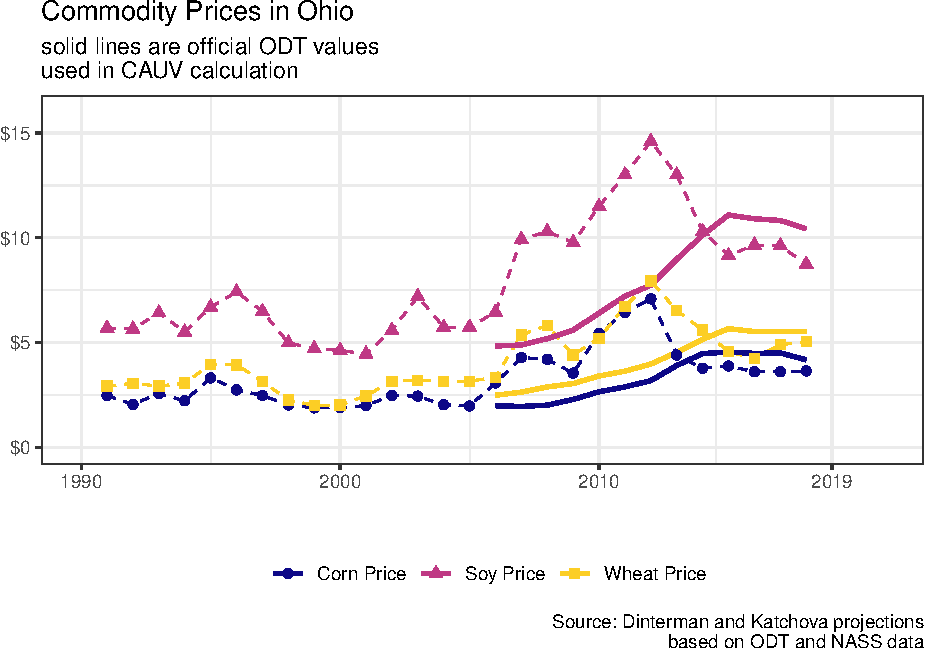
\includegraphics[width=1\linewidth]{4-projections-2019-2020_files/figure-latex/viz-prices-1} \caption{\label{fig:prices}}\label{fig:viz-prices}
\end{figure}

In the event that the high or low values of our projected commodity
prices arises, we have calculated those scenarios for historical price
data in the following tables:

\begin{longtable}[]{@{}rlllll@{}}
\caption{Historical Corn Prices}\tabularnewline
\toprule
Year & ODT Price & USDA Price & Projection & Low Projection & High
Projection\tabularnewline
\midrule
\endfirsthead
\toprule
Year & ODT Price & USDA Price & Projection & Low Projection & High
Projection\tabularnewline
\midrule
\endhead
2011 & \$2.89 & \$6.44 & \$2.89 & \$2.57 & \$3.05\tabularnewline
2012 & \$3.19 & \$7.09 & \$3.26 & \$2.80 & \$3.26\tabularnewline
2013 & \$3.91 & \$4.41 & \$3.93 & \$3.26 & \$3.93\tabularnewline
2014 & \$4.48 & \$3.78 & \$4.54 & \$3.93 & \$4.54\tabularnewline
2015 & \$4.55 & \$3.89 & \$4.57 & \$4.55 & \$5.18\tabularnewline
2016 & \$4.49 & \$3.61 & \$4.50 & \$4.42 & \$5.00\tabularnewline
2017 & \$4.51 & \$3.61 & \$4.50 & \$4.50 & \$5.09\tabularnewline
2018 & \$4.18 & \$3.65 & \$4.16 & \$4.17 & \$4.73\tabularnewline
2019 & \$NA & \$NA & \$3.68 & \$3.68 & \$4.22\tabularnewline
2020 & \$NA & \$NA & \$3.53 & \$3.52 & \$3.68\tabularnewline
\bottomrule
\end{longtable}

\begin{longtable}[]{@{}rlllll@{}}
\caption{Historical Soybean Prices}\tabularnewline
\toprule
Year & ODT Price & USDA Price & Projection & Low Projection & High
Projection\tabularnewline
\midrule
\endfirsthead
\toprule
Year & ODT Price & USDA Price & Projection & Low Projection & High
Projection\tabularnewline
\midrule
\endhead
2011 & \$7.22 & \$13.00 & \$7.45 & \$6.63 & \$7.42\tabularnewline
2012 & \$7.74 & \$14.60 & \$7.93 & \$7.16 & \$7.93\tabularnewline
2013 & \$8.98 & \$13.00 & \$9.08 & \$7.94 & \$9.08\tabularnewline
2014 & \$10.13 & \$10.30 & \$10.40 & \$9.08 & \$10.40\tabularnewline
2015 & \$11.09 & \$9.16 & \$11.08 & \$11.00 & \$11.95\tabularnewline
2016 & \$10.91 & \$9.66 & \$10.91 & \$10.91 & \$11.78\tabularnewline
2017 & \$10.83 & \$9.62 & \$10.83 & \$10.77 & \$11.78\tabularnewline
2018 & \$10.43 & \$8.75 & \$10.46 & \$10.38 & \$11.35\tabularnewline
2019 & \$NA & \$NA & \$9.78 & \$9.78 & \$10.70\tabularnewline
2020 & \$NA & \$NA & \$9.00 & \$9.00 & \$9.78\tabularnewline
\bottomrule
\end{longtable}

\begin{longtable}[]{@{}rlllll@{}}
\caption{Historical Wheat Prices}\tabularnewline
\toprule
Year & ODT Price & USDA Price & Projection & Low Projection & High
Projection\tabularnewline
\midrule
\endfirsthead
\toprule
Year & ODT Price & USDA Price & Projection & Low Projection & High
Projection\tabularnewline
\midrule
\endhead
2011 & \$3.64 & \$6.73 & \$3.62 & \$3.37 & \$3.95\tabularnewline
2012 & \$3.98 & \$7.94 & \$3.96 & \$3.64 & \$4.20\tabularnewline
2013 & \$4.54 & \$6.54 & \$4.55 & \$3.96 & \$4.55\tabularnewline
2014 & \$5.16 & \$5.60 & \$5.19 & \$4.55 & \$5.19\tabularnewline
2015 & \$5.67 & \$4.57 & \$5.69 & \$5.38 & \$5.99\tabularnewline
2016 & \$5.53 & \$4.25 & \$5.53 & \$5.32 & \$6.02\tabularnewline
2017 & \$5.53 & \$4.90 & \$5.53 & \$5.53 & \$6.02\tabularnewline
2018 & \$5.52 & \$5.05 & \$5.51 & \$5.33 & \$5.97\tabularnewline
2019 & \$NA & \$NA & \$5.15 & \$4.96 & \$5.62\tabularnewline
2020 & \$NA & \$NA & \$4.81 & \$4.62 & \$5.15\tabularnewline
\bottomrule
\end{longtable}

\hypertarget{yield}{%
\subsubsection{Yield}\label{yield}}

Each soil type has a corresponding base yield of production for each
commodity from 1984 -- which is the most recent comprehensive soil
survey for the state of Ohio and separate from the base yield of
non-land costs. Prior to 2006, ODT did not adjust for yield trends and
calculated gross operating income for each soil type via their 1984
yields which suppressed revenues -- in the formula this would
effectively mean that the \(Yield_{c,Ohio,t}\) equaled
\(Yield_{c,Ohio,1984}\).

ODT began adjusting for yield trends through the current method of
taking the 7-year averages of state-wide yields (irrespective of soil
type), dividing by the state-wide yields for each commodity in 1984,
then multiplying this value based on the 1984 commodity yield for the
particular soil type evaluated. This can be thought of as an adustment
factor to account for the general trend of increasing yields in corn,
wheat, and soybeans. Prior to 2014, the 7-year calculation involved a
two year lag -- i.e.~the 2014 tax year used average yield values from
2003 through 2012. In 2015 and beyond, there is only a one year lag --
i.e.~2015 tax year used average yield values from 2005 through 2014.

The values for commodity yields for tax year 2019 are known because USDA
has published their 2018 values for each commodity -- however for
unknown future values we use the 30-year yield trend. The yield values
for the 2019 CAUV calculations are 163 for corn, 50.4 for soybeans, and
69.7 for wheat. Our yield projections for the 2020 CAUV calculations are
163.2 for corn, 50.8 for soybeans, and 70.1 for wheat. These historical
yield trends are displayed in figure \ref{fig:yields} and in the
following tables:

\begin{figure}[H]
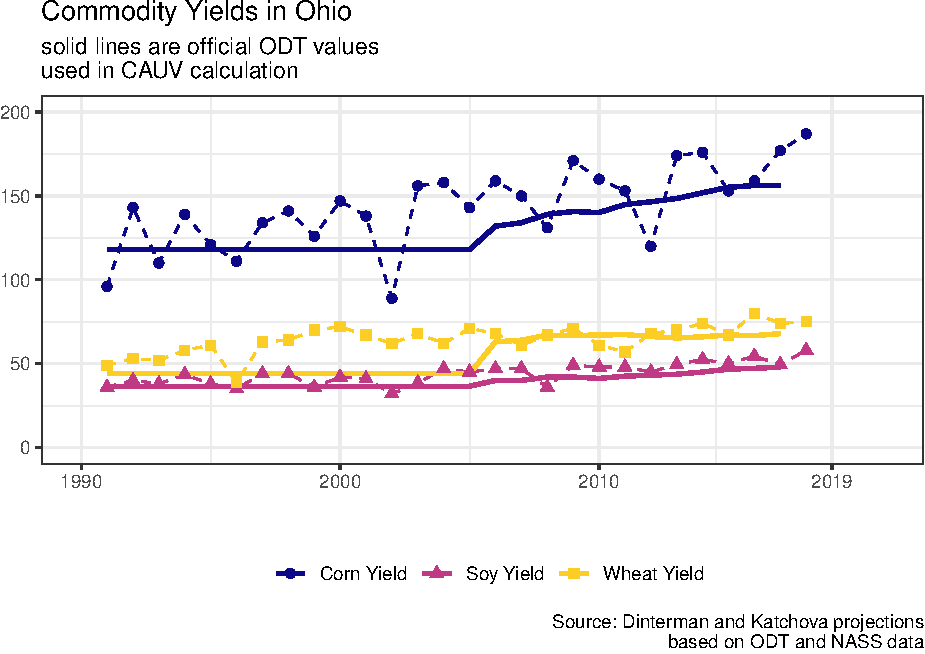
\includegraphics[width=1\linewidth]{4-projections-2019-2020_files/figure-latex/viz-yields-1} \caption{\label{fig:yields}}\label{fig:viz-yields}
\end{figure}

\newpage

\begin{longtable}[]{@{}rrrr@{}}
\caption{Historical Corn Yields}\tabularnewline
\toprule
Year & ODT Yield & USDA Yield & Projected Yield\tabularnewline
\midrule
\endfirsthead
\toprule
Year & ODT Yield & USDA Yield & Projected Yield\tabularnewline
\midrule
\endhead
2007 & 134.0 & 150 & 134.3\tabularnewline
2008 & 139.0 & 131 & 139.1\tabularnewline
2009 & 140.7 & 171 & 140.7\tabularnewline
2010 & 140.1 & 160 & 139.7\tabularnewline
2011 & 144.9 & 153 & 144.2\tabularnewline
2012 & 146.5 & 120 & 145.5\tabularnewline
2013 & 148.5 & 174 & 147.0\tabularnewline
2014 & 151.9 & 176 & 150.1\tabularnewline
2015 & 155.2 & 153 & 153.7\tabularnewline
2016 & 156.2 & 159 & 154.7\tabularnewline
2017 & 156.2 & 177 & 154.7\tabularnewline
2018 & 158.9 & 187 & 157.4\tabularnewline
2019 & NA & NA & 163.0\tabularnewline
2020 & NA & NA & 163.2\tabularnewline
\bottomrule
\end{longtable}

\begin{longtable}[]{@{}rrrr@{}}
\caption{Historical Soybean Yields}\tabularnewline
\toprule
Year & ODT Yield & USDA Yield & Projected Yield\tabularnewline
\midrule
\endfirsthead
\toprule
Year & ODT Yield & USDA Yield & Projected Yield\tabularnewline
\midrule
\endhead
2007 & 40.0 & 47.0 & 40.5\tabularnewline
2008 & 42.0 & 36.0 & 41.6\tabularnewline
2009 & 42.0 & 49.0 & 42.0\tabularnewline
2010 & 41.2 & 48.0 & 41.1\tabularnewline
2011 & 42.5 & 48.0 & 42.5\tabularnewline
2012 & 43.1 & 45.0 & 43.0\tabularnewline
2013 & 43.7 & 49.5 & 43.8\tabularnewline
2014 & 45.0 & 52.5 & 45.0\tabularnewline
2015 & 46.7 & 50.0 & 46.7\tabularnewline
2016 & 47.2 & 54.5 & 47.2\tabularnewline
2017 & 47.9 & 49.5 & 48.0\tabularnewline
2018 & 48.2 & 58.0 & 48.2\tabularnewline
2019 & NA & NA & 50.4\tabularnewline
2020 & NA & NA & 50.8\tabularnewline
\bottomrule
\end{longtable}

\begin{longtable}[]{@{}rrrr@{}}
\caption{Historical Wheat Yields}\tabularnewline
\toprule
Year & ODT Yield & USDA Yield & Projected Yield\tabularnewline
\midrule
\endfirsthead
\toprule
Year & ODT Yield & USDA Yield & Projected Yield\tabularnewline
\midrule
\endhead
2007 & 64.0 & 61 & 63.8\tabularnewline
2008 & 67.0 & 67 & 66.7\tabularnewline
2009 & 66.7 & 71 & 66.5\tabularnewline
2010 & 67.1 & 61 & 66.8\tabularnewline
2011 & 67.3 & 57 & 66.9\tabularnewline
2012 & 66.2 & 68 & 65.8\tabularnewline
2013 & 65.3 & 70 & 64.8\tabularnewline
2014 & 66.0 & 74 & 65.4\tabularnewline
2015 & 67.1 & 67 & 66.8\tabularnewline
2016 & 66.7 & 80 & 66.4\tabularnewline
2017 & 67.9 & 74 & 67.6\tabularnewline
2018 & 69.2 & 75 & 68.9\tabularnewline
2019 & NA & NA & 69.7\tabularnewline
2020 & NA & NA & 70.1\tabularnewline
\bottomrule
\end{longtable}

\hypertarget{capitalization-rate}{%
\subsection{Capitalization Rate}\label{capitalization-rate}}

Of the factors going into the CAUV calculation, the capitalization rate
is in the denominator of the equation and has a significant impact on
overall CAUV values because of it's relatively small value and range
(see historical values in the next section). The economic purpose of a
capitalization rate is to capture the future stream of revenues form an
asset into a present value and thus the capitalization rate acts as an
interest rate.

Prior to 2015, the capitalization rate was based on a 60\% loan and 40\%
equity appreciation with interest rates for each value based on a 7-year
Olympic average where the value for the loan interest rate came from a
15-year mortgage from Farm Credit Services (FCS) and the equity interest
rate was the Federal Funds rate plus two percentage points. Both of
these interest rates use the current tax year's value in calculation so
the value calculated for 2014 was an Olympic average over the years 2008
through 2014. This loan/equity mix is calculated and then 5 years of
equity buildup and appreciation are subtracted from the interest rate
plus a tax additur -- the average effective tax rate for agricultural
land applied at 35\% of the market value.

For the 2015 tax year, the capitalization rate changed to an 80\% loan
(based on 25-year mortgage from FCS) and 20\% equity appreciation. Then
in 2017, ODT changed the interest rate used for equity Economic Research
Services (ERS) -- this amount is lagged two years so the 2017 value is
based on 1991 through 2015 values. The loan interest rate remains a
7-year Olympic average that is not lagged, so the 2017 interest rate
used values from 2011 through 2017. The formula dropped appreciation
from calculations and changed the equity buildup calculation from 5
years to 25 years.

The capitalization rate requires the knowledge of an interest rate on a
loan and an equity rate as well as the term and debt percentage for
determining from the
\href{http://www.commercialappraisalsoftware.dcfsoftware.com/mtgequity.htm}{Mortgage-Equity
Method}. But it can be defined as:

\[ \begin{aligned}
{CAP_t} &= {Loan \%}_t \times {Annual Debt Service}_t + \\
& {Equity \%}_t \times {Equity Yield}_t - \nonumber \\
& {Buildup}_t + \nonumber \\
& {Tax Additur Adjustment}_t
\end{aligned} \]

The \({Loan \%}_t\) plus \({Equity \%}_t\) must equal one and is
currently an 80\% to 20\% ratio respectively. Prior to 2015, the values
were based on 60\% loan and 40\% equity appreciation.

\({Annual Debt Service}_t\) is a debt servicing factor based on a
25-year term mortgage with an associated interest rate. The interest
rate used for a particular year is based on a 7-year Olympic average
where the value for the loan interest rate came from a 25-year mortgage
from FCS. Prior to 2015, a 15-year term was used instead of 25 and there
were no lags in this formula. For example, the 2017 interest rate used
comes from FCS values between 2011 and 2017. The formula for calculating
the debt servicing factor with \(r\) as the interest rate (from FCS) and
\(n\) the term length (currently 25) is:

\[ {Annual Debt Service} = \frac{r \times (1 + r)^n}{(1 + r)^n - 1} \]

Next, the \({Equity Yield}_t\) needs to be calculated -- which is simply
the interest rate associated with equity that a farmer may hold. Prior
to 2017, the equity yield was a 7-year Olympic average of the prime rate
plus 2\% from the Wall Street Journal's bank survey -- with no lag for
the values. In 2017, the ODT switched the equity yield to be a two year
lagged 25-year average of the ``Total rate of return on farm equity''
from the \href{https://data.ers.usda.gov/reports.aspx?ID=17838}{Economic
Research Services} of the USDA. For example, the 2017 value used the
ERS's values from 1991 to 2015.

Then, the equity buildup associated with a set time frame needs to be
calculated. The equity buildup formula involves an associated interest
rate (the \({Equity Yield}_t\) is used here as \(r\)) and a time-frame
\(n\), which is set at 25 years currently (prior to 2017, this was set
at 5 years of equity buildup):

\[ {Buildup}_t = {Equity \%}_t \times {Mortgage Paid \%}_t \times \frac{r}{(1 + r)^n - 1} \]

For 2017 and beyond, the \({Mortgage Paid \%}_t\) is assumed to be
100\%. However, prior to 2017 this value needed to be calculated as the
percentage of mortgage paid after 5 years. The mortgage term was needed
to determine what the mortgage paid after 5 years would be. For 2015 and
beyond the mortgage terms have been for 25 years while prior to 2015 the
mortgage term was for 15 years. The formula for calculating the
percentage of the mortgage paid off after 5 years is:

\[ {Mortgage Paid \%}_t = \frac{ \frac{1}{ (1 + r)^{n-5} } - \frac{1}{ (1 + r)^n} }{ 1 - \frac{1}{(1 + r)^n} } \]

Where \(r\) is the interest rate and \(n\) is the term of the loan.

And finally, the \({Tax Additur Adjustment}_t\) needs to be calculated.
The tax additur is added onto the capitalization rate as a way to proxy
for property taxes as a ratio to market value. The statewide average
effective tax rate on agricultural land, as determined through table
\href{https://www.tax.ohio.gov/tax_analysis/tax_data_series/publications_tds_property.aspx\#Allpropertytaxes}{DTE27},
from the previous tax year is used in calculation for the tax additur in
question. The statewide average effective tax rate is expressed in terms
of mills and the tax additur is then expressed as:

\[ {Tax Additur Adjustment}_t = \frac{0.35 \times {Statewide Millage}_{t-1} }{1000} \]

The tax additur component remained in the calculation and between 2006
and 2017 it ranged from 1.30\% to 1.60\%.

\hypertarget{capitalization-rate-values}{%
\subsection{Capitalization Rate
Values}\label{capitalization-rate-values}}

The capitalization rates used by the ODT in CAUV calculations since 2003
are displayed in figure \ref{fig:viz-cap}, which shows a steady decline
until the formula change in 2015. The projected capitalization rate for
2019 is 8.0\% and in 2020 the projected value is 8.0\%.

In addition, the scenarios for a ``high'' and ``low'' capitalization
rate in 2019 and 2020 are numerically displayed in red and blue
respectively. A ``high'' scenario implies the highest potential CAUV
values, which would be a lower capitalization rate because the
capitalization rate is in the denominator of the formula for CAUV.
Vice-versa for the ``low'' projection of CAUV value. These scenarios
utilize the Olympic averages which will always drop the highest and
lowest values for the previous 7 years. Since the 2019 FCS interest is
unknown, the ``high'' (``low'') scenario assumes that the 2019 interest
rate will be 0 (infinite) and calculates the value used in ODT
calculations for this. The ``high'' value of our projected
capitalization rate of 7.80\% leads to a high CAUV value whereas our
capitalization rate is 8.14\% for a ``low'' CAUV value.

Of the capitalization rate projections, only the tax additur and FCS
interest rate are currently unknown for 2019 and beyond. The equity
appreciation rate is already known because USDA-ERS has published their
2017 value for total rate of return on farm equity -- thus allowing for
the 2019 tax year calculation. The 25-year mortgage from FCS uses a
7-year Olympic average, which allows for a ``high'' and ``low'' CAUV
value projection. The tax additur is reported by the ODT for that
particular tax year -- in lieu of utilizing the Olympic average and this
projection uses a +/- 0.1\% range with the tax additur from the 2018
value.

\begin{longtable}[]{@{}rllll@{}}
\caption{Historical Capitalization Rates}\tabularnewline
\toprule
Year & ODT Value & Projected & Low & High\tabularnewline
\midrule
\endfirsthead
\toprule
Year & ODT Value & Projected & Low & High\tabularnewline
\midrule
\endhead
2010 & 7.8\% & 7.8\% & 8.0\% & 7.7\%\tabularnewline
2011 & 7.6\% & 7.6\% & 7.8\% & 7.4\%\tabularnewline
2012 & 7.5\% & 7.5\% & 7.7\% & 7.2\%\tabularnewline
2013 & 6.7\% & 6.7\% & 7.0\% & 6.6\%\tabularnewline
2014 & 6.2\% & 6.2\% & 6.6\% & 6.2\%\tabularnewline
2015 & 6.6\% & 6.6\% & 6.9\% & 6.4\%\tabularnewline
2016 & 6.3\% & 6.3\% & 6.6\% & 6.2\%\tabularnewline
2017 & 8.0\% & 8.0\% & 8.2\% & 7.8\%\tabularnewline
2018 & 8.0\% & 8.0\% & 8.1\% & 7.8\%\tabularnewline
2019 & NA\% & 8.0\% & 8.1\% & 7.8\%\tabularnewline
2020 & NA\% & 8.0\% & 8.1\% & 7.8\%\tabularnewline
\bottomrule
\end{longtable}

\newpage

\hypertarget{cauv-values}{%
\section{CAUV Values}\label{cauv-values}}

\hypertarget{cauv-values-by-soil-type}{%
\subsection{CAUV Values by Soil Type}\label{cauv-values-by-soil-type}}

Effectively, every soil type throughout Ohio is assigned a CAUV value
each year that is dependent on average corn, soybeans, and wheat
revenues less costs over the previous 7 to 10 years. Soil types that
have higher productive capacity -- based on 1984 values -- will have
higher CAUV values than those with lower productivity. However, some
soil types are relatively more productive with respect to one commodity
than the others.

ODT provides a comprehensive soil productivity index for every soil type
in Ohio based upon relative yields of corn, soybeans, wheat, oats, and
hay across the state of Ohio. The index ranges from 0 to 100 and
provides a barometer for how productive soil types across the state are.
Figure \ref{fig:cropland-trend} places soil types in bins according to
their productivity index and plots the average CAUV value since 1991 to
provide a range of CAUV values. ODT provides an additional mandate for a
minimum CAUV value. Prior to 2009, this was \$100 but the value
subsequently rose to \$170, \$200, \$300, and finally \$350 in 2012. The
most recent official values from ODT are from 2018, which are displayed
in figure \ref{fig:cropland-trend}:

\begin{figure}[H]
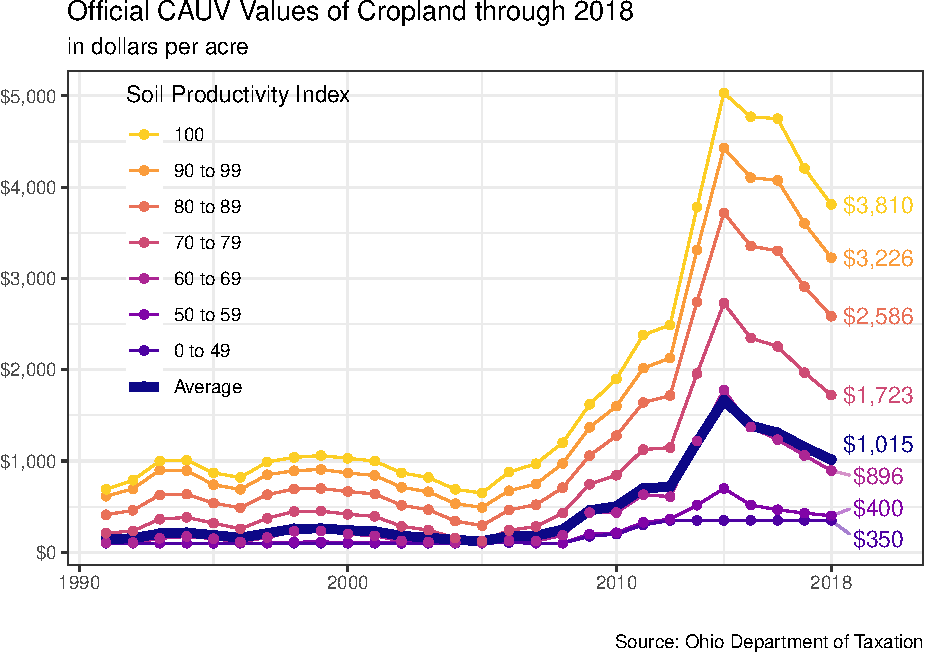
\includegraphics[width=1\linewidth]{4-projections-2019-2020_files/figure-latex/cropland-trend-1} \caption{\label{fig:cropland-trend}}\label{fig:cropland-trend}
\end{figure}

\hypertarget{phase-in}{%
\subsection{Phase-In}\label{phase-in}}

Part of the legislative changes to the CAUV formula in 2017 was that the
change in CAUV values would be phased in over time. The 2017 values had
an adjustment factor where only half of the difference were added on
between the 2016 CAUV value and what the pre-adjusted 2017 CAUV would
have been. Figure \ref{fig:phase-in} displays how the phase-in
legislation affected the 2018 CAUV values across different soil types:

\begin{figure}[H]
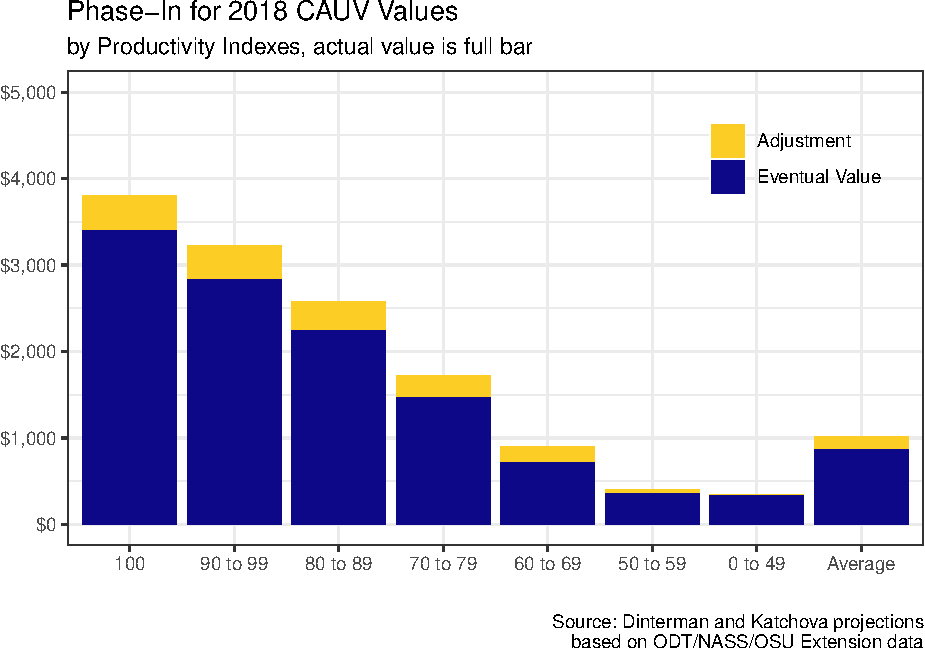
\includegraphics[width=1\linewidth]{4-projections-2019-2020_files/figure-latex/phase-in-1} \caption{\label{fig:phase-in}}\label{fig:phase-in}
\end{figure}

Low productivity soils were largely unaffected as many of the lowest
quality soils were at the minimum value for both 2016 and 2017 -- \$350.
While the average value across all soil types in 2018 was \$1,015, the
adjustment associated with the phase-in period accounted for \$140 on
average. If the phase-in period was not in effect, the average CAUV
value would have been \$874.

\hypertarget{possible-ranges}{%
\subsection{Possible Ranges}\label{possible-ranges}}

While our expected projections are noted at the beginning of this
report, we also provide the high and low potential projections for both
2019 and 2020.

\hypertarget{high-2019}{%
\subsubsection{High 2019}\label{high-2019}}

\begin{figure}[H]
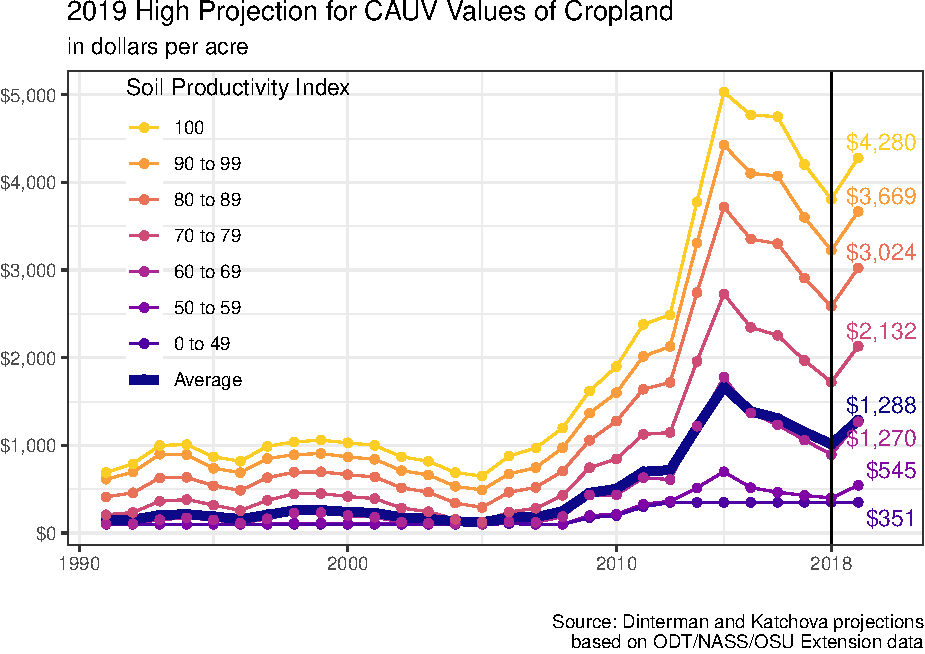
\includegraphics[width=1\linewidth]{4-projections-2019-2020_files/figure-latex/high-trend-1} \caption{\label{fig:high-trend}}\label{fig:high-trend}
\end{figure}

\hypertarget{low-2019}{%
\subsubsection{Low 2019}\label{low-2019}}

\begin{figure}[H]
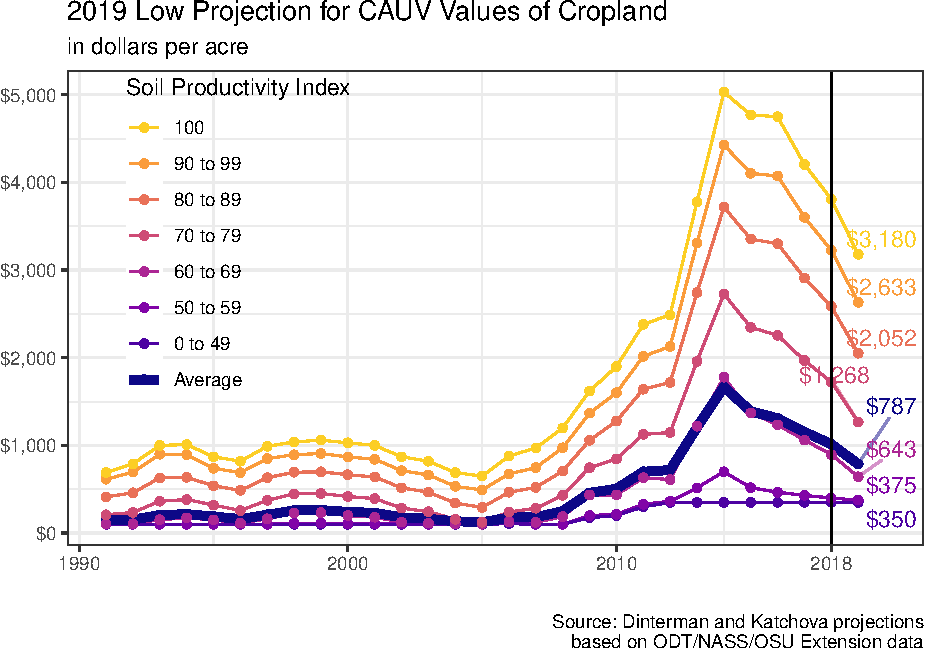
\includegraphics[width=1\linewidth]{4-projections-2019-2020_files/figure-latex/low-trend-1} \caption{\label{fig:low-trend}}\label{fig:low-trend}
\end{figure}

\hypertarget{high-2020}{%
\subsubsection{High 2020}\label{high-2020}}

\begin{figure}[H]
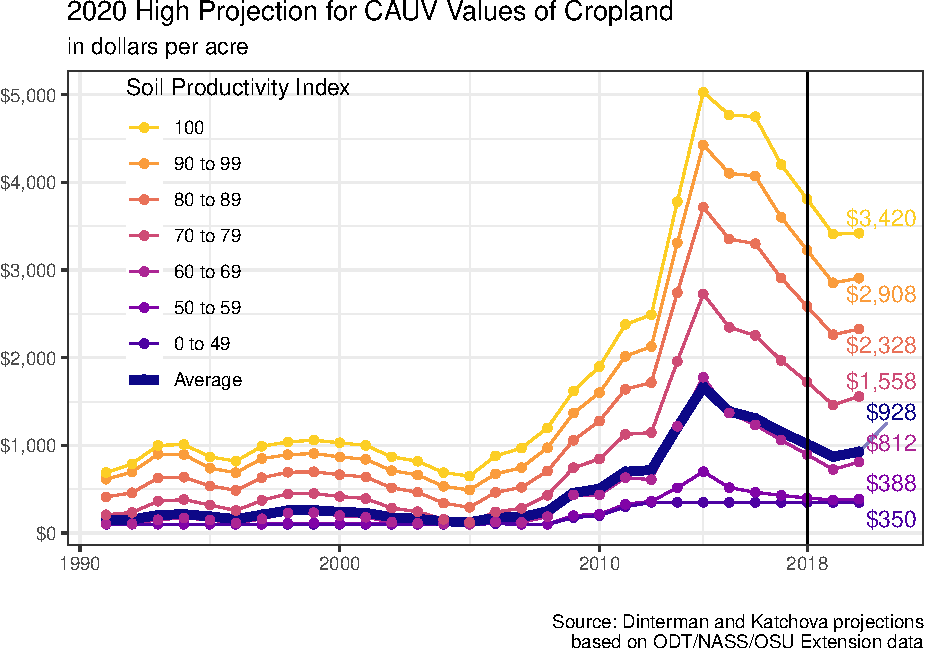
\includegraphics[width=1\linewidth]{4-projections-2019-2020_files/figure-latex/high-trend-2020-1} \caption{\label{fig:high-trend-2020}}\label{fig:high-trend-2020}
\end{figure}

\hypertarget{low-2020}{%
\subsubsection{Low 2020}\label{low-2020}}

\begin{figure}[H]
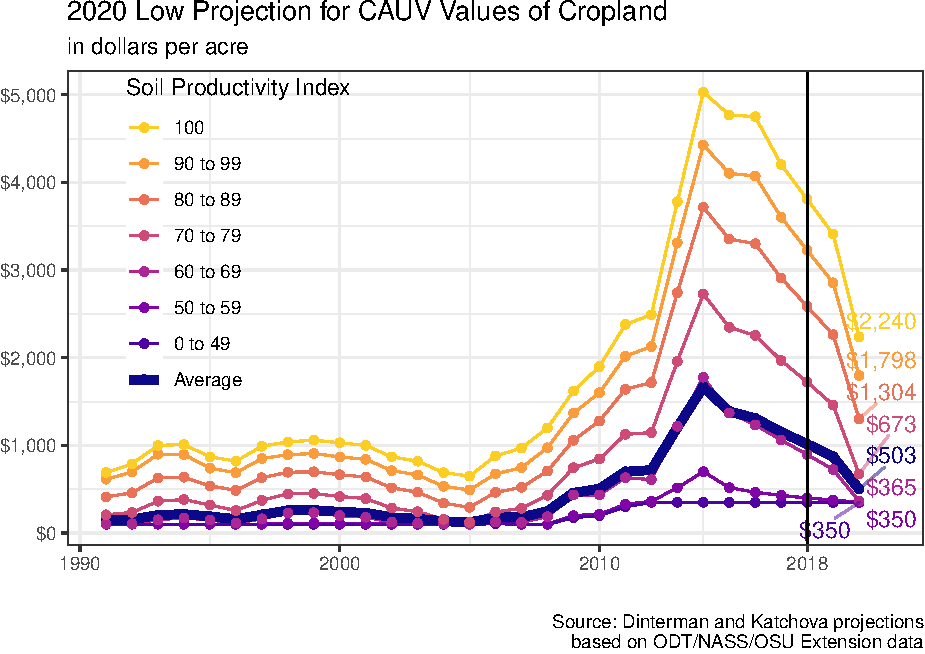
\includegraphics[width=1\linewidth]{4-projections-2019-2020_files/figure-latex/low-trend-2020-1} \caption{\label{fig:low-trend-2020}}\label{fig:low-trend-2020}
\end{figure}

\hypertarget{references}{%
\section{References}\label{references}}

\begin{itemize}
\tightlist
\item
  Farm Office annual crop budget reports
  \url{https://farmoffice.osu.edu/farm-management-tools/farm-budgets}
\item
  Ohio Code of Legislation \url{http://codes.ohio.gov/orc/5713.31} and
  \url{http://codes.ohio.gov/orc/5715.01}
\item
  ODT CAUV Information page
  \url{https://www.tax.ohio.gov/real_property/cauv.aspx}
\item
  USDA-NASS price and yield data \url{https://quickstats.nass.usda.gov}
\item
  USDA-ERS total rate of return on farm equity data
  \url{https://www.ers.usda.gov/data-products/farm-income-and-wealth-statistics/data-files-us-and-state-level-farm-income-and-wealth-statistics/}
\end{itemize}

Projections for 2019 CAUV values are available at
\url{https://aede.osu.edu/file/cauvprojections2019.xlsx}

Projections for 2020 CAUV values are available at
\url{https://aede.osu.edu/file/cauvprojections2020.xlsx}


\end{document}
